\documentclass[notitlepage]{article}
\usepackage[utf8]{inputenc} 
\usepackage{geometry} 		
\usepackage{chngcntr}
\usepackage{amsmath} 			
\usepackage{amssymb}			
\usepackage{mathtools}		
\usepackage{comment} 			
\usepackage{mdframed}			
\usepackage{xcolor}				
\usepackage{fancyhdr}			
\usepackage{listings}			
\usepackage{color}				
\usepackage{tikz}	
\usepackage{tasks}			
\usepackage{exsheets}		
\usepackage{array}		
\usepackage{graphicx}	
\usepackage{empheq}
\usepackage{caption}
\usepackage{pdfpages}
\usepackage{tabularx}

\geometry{ 						%Format titlepage (interrupted by newgeometry)
	a4paper,
	total={170mm,257mm}%,
	%left=0mm,
	%top=0mm,
}

%START DEFINE YOUR VARIABLES HERE

\newcommand{\documentName}{Requirement Specification Document}
\newcommand{\projectName}{Label Refinement by Behavioral Similarity}

%END DEFINE YOUR VARIABLES HERE

\title{%
	\documentName\text{ } \\
  \large \projectName\text{ } \\
  }

\author{
	\large \underline{Document owners:}\\ 
	Bianka Bakullari\\
	\texttt{}
	Christopher Beine\\
	\texttt{}
	Nicole Ventsch\\
	\texttt{}
	Juan\\
	\texttt{}
}

\date{\small{Last edited: \today}}

\pagestyle{fancy}
\fancyhf{}
\rhead{}
\lhead{\documentName\space-\space\projectName}

\makeatletter					%Prefix to add ToC to titlepage
\newcommand*{\toccontents}{\@starttoc{toc}}
\renewcommand*\contentsname{}
\makeatother
                  

\begin{document}

\begin{titlepage}
\clearpage\maketitle			%Clear title page
\thispagestyle{fancy}


\end{titlepage}

\title{ \large \textbf{ Contents}}
\tableofcontents

\newpage

\rfoot{\thepage}				%Start printing page-numbers, after title page.

\newgeometry{ 					%Default page formatting on-going #1
	total={170mm,257mm},
	left=20mm,
	top=25mm,
    bottom=30mm					%Causes warning
}

\begin{flushleft}				%Default page formatting on-going #2

\section{Project Drivers}

\subsection{The Purpose of the Project}

The purpose of the project is providing a platform that allows refinements of event logs, where activities that originally had the same label are relabelled if they have different structural behaviours. In order to do so, an interactive web service should be implemented which allows users to upload event logs in the standard XES or CSV format and set thresholds for the refinements. This event log should contain activities that are carried out multiple times and are named identically. The web service should then apply the refinement algorithm and finally, the user should be able to download the refined event log in XES format. By using the refinement algorithm, more accurate and precise BPMs (Business Process Models) are generated which provides better insights into the processes.

\subsection{The Client, the Customer and other Stakeholders}

The client of this project is the Chair of Process and Data Science at the RWTH Aachen, which provides the supervision and support for this project. Furthermore, there are many different potential users. For example, students or researchers could use the website as a pre-processing step in order to continue research with the refined log. Additionally, business analysts from companies could use it in order to get a better insight from the refined log than from the original one. Since we will provide a web service, it will be easily accessed and not bound to an specific type of user. 

\section{Project Constraints}

\subsection{Mandated Constraints}

\subsection{Naming Conventions and Definitions}

\subsection{Relevant Facts and Assumptions}


\section{Functional Requirements}

\subsection{The Scope of the Work}
As explained in the Project Initiation document, we aim to provide a web application where the end user can apply the Label Refinement automatically as a pre-processing step to his event log.
The new and refined log could later be used as alternative input for process discovery algorithms in other tools, yielding a new model and thus adding an alternative to the solution space of possible process models.


\subsection{The Scope of the Product}
The final product consists of a web interface where the user can upload event logs, parameterize thresholds and then the Label Refinement algorithm is executed. 
In order to get an overview of the product, a use case analysis was carried out, where we identify the system actors and their functions. 
Since the project's focus is the Label Refinement implementation, the project was divided into two systems. 
This allows a better visualisation of the individual algorithm steps and system interactions. The following use cases were identified within the analysis.\\
\medskip
Figure \ref{fig:front-end} displays the Use Cases for the final web interface and thus the system interactions with the end-user.  
Figure \ref{fig:back-end} indicates the Use Cases of, which are required for the Label Refinement algorithm. So the front-end diagram refers to UI functions  
and the back-end diagram to a more technical view.
\begin{figure}[h!]
  \includegraphics[width=\textwidth]{"UML Files/Use Case Diagram front-end".png}
  \caption{Use cases front-end}
  \label{fig:front-end}
\end{figure}

\begin{figure}[h!]
  \includegraphics[width=\textwidth]{"UML Files/Use Case Diagram back-end".png}
  \caption{Use cases backen-end}
  \label{fig:back-end}
\end{figure}
\clearpage
The following actors exists in the final system:\\
\medskip
\begin{tabularx}{\textwidth}{|m{4cm}|m{4cm}|m{8cm}|}
	\hline
	\textbf{Actor} 
	&\textbf{Symbol}
	&\textbf{Description}\\
	\hline
	End user & \includegraphics[width=60px, height=75px]{"UML Files/enduser".png} & The End user interacts with the web interface of the system and does not need any information about the technical implementation\\
	\hline
	Webclient & \includegraphics[width=100px]{"UML Files/webclient".png} & The Webclient provides the API access on simple abstraction layer to provide an easy algorithm execution\\
	\hline
	Event Label Refining Front-end & \includegraphics[width=100px]{"UML Files/front-end".png} & The Event Label Refining Front-end is the Webclient which is delivered with the project \\
	\hline
	Event Label Refining Back-end & \includegraphics[width=100px]{"UML Files/back-end".png} & The Event Label Refining Backend-end is responsible for label refining algorithm. It provides access via an API \\
	\hline
\end{tabularx}

\subsection{Functional and Data Requirements}
The following requirements result from the use case analysis:\\
\medskip
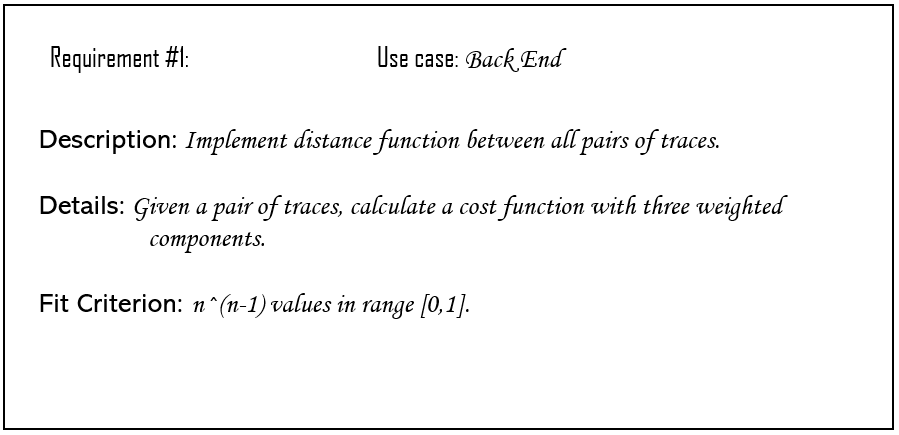
\includegraphics[scale=0.6]{Req1.png}

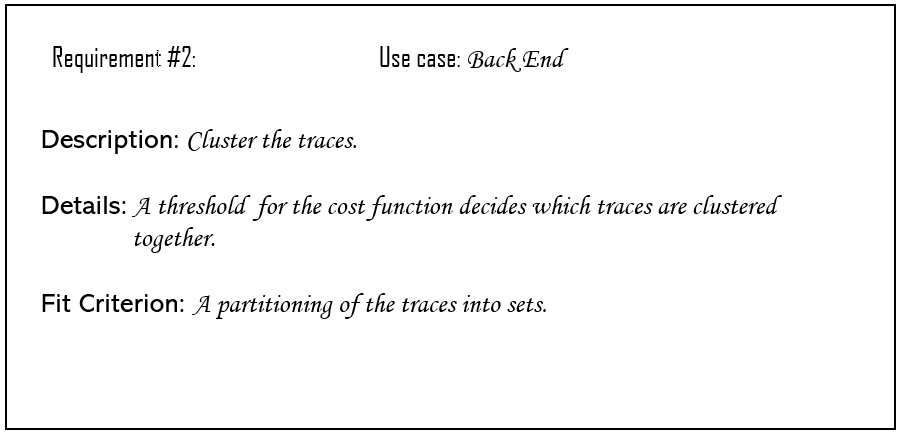
\includegraphics[scale=0.6]{Req2.png}

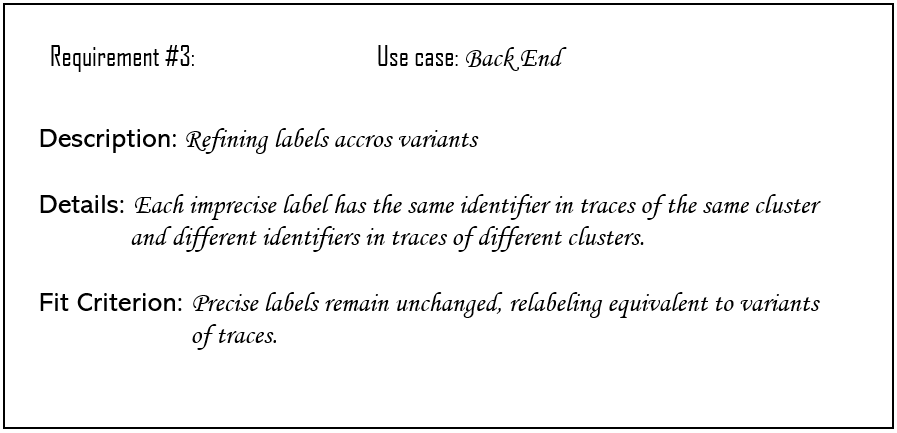
\includegraphics[scale=0.6]{Req3.png}

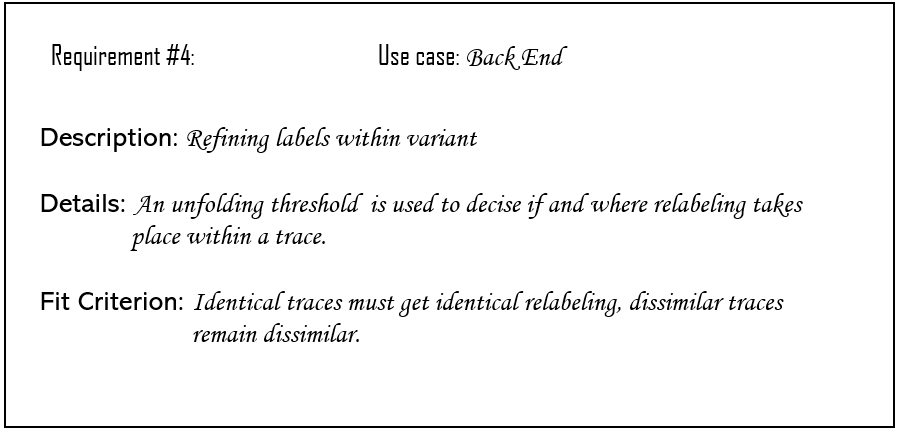
\includegraphics[scale=0.6]{Req4.png}

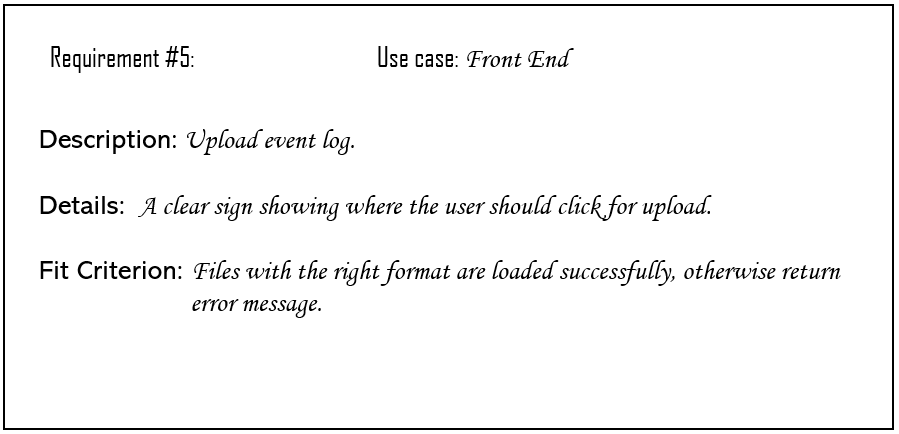
\includegraphics[scale=0.6]{Req5.png}

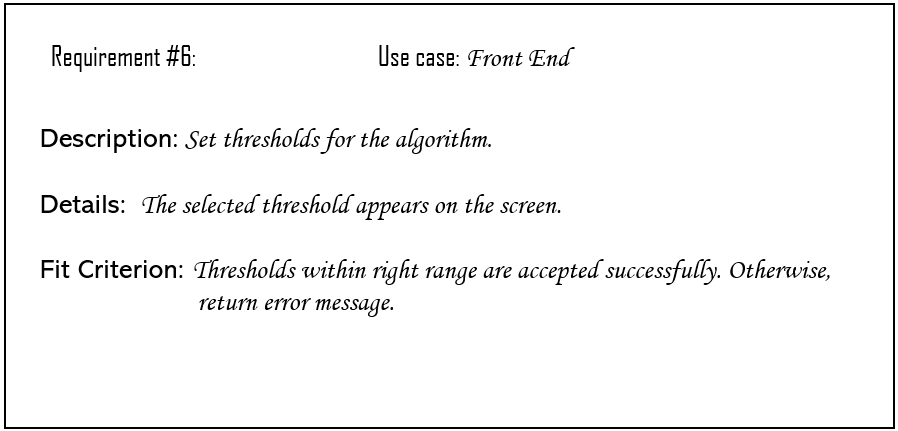
\includegraphics[scale=0.6]{Req6.png}

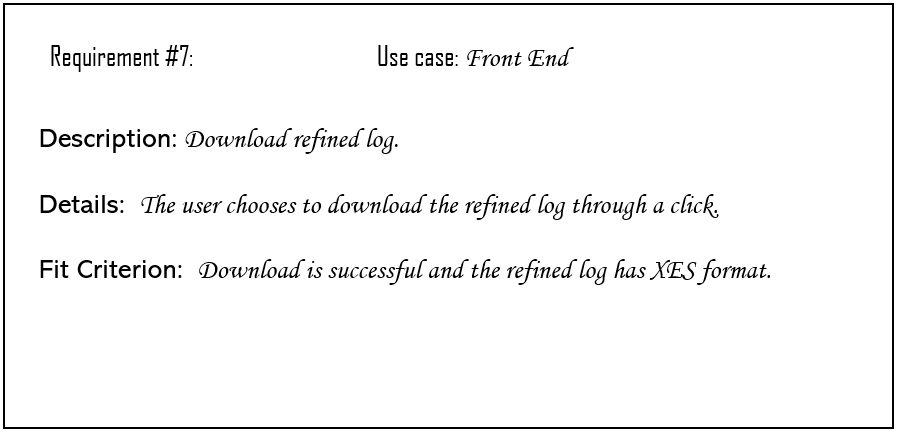
\includegraphics[scale=0.6]{Req7.png}




\section{Nonfunctional Requirements}

\subsection{Look and Feel Requirements and Usability}
The user interface must be self-explanatory and easy to use.
It should be clear where the event log can be uploaded and/or downloaded.
For each threshold, the user should be able to type in his choice and see it on the screen.
In case that the event log has the wrong format or the chosen threshold is out of range, an error message displayed on the screen should imply what has gone wrong.

Our product is aimed at users who have some knowledge in Process Mining, are familiar with the algorithm or are previously informed about the concept and effects of relabeling.




%\subsection{Performance Requirements}

\subsection{Operational and Environmental Requirements}
The project must meet the following technical requirements:
\medskip
\begin{itemize}
	\item Back-end must be deployable on a production-grade server.
	\item Front-end must be deployable on production-grade server.
	\item Front-end must support Google Chrome (Version $\geq$ 65) and Mozilla Firefox (Version $\geq$ 60).
\end{itemize}
\medskip
To validate the Operational and Environmental requirements, the front-end requirements are tested in Mozilla Firefox and Google Chrome. 
\subsection{Maintainability and Support Requirements}
After finishing the project, the web service should be self-explanatory for the users. We do not intent to offer support other than documentation to the users. Moreover, the website should only include the aspects we mentioned above and is not intended to be expanded by us after this project. We do not intend maintaining the web service after finishing this project.
\section{Project Issues}

\subsection{Open Issues}
Our team has a rough idea of the steps needed to implement the algorithm and the interface.
However, we are unsure about the relative time needed for each of these components.
During the implementation of the algorithm, many unexpected bugs might show up and could hinder the time we have in our disposal to design a user-friendly web-interface.

While we will strive to write an efficient algorithm, there are no guarantees about its  performance when the number of requests increases beyond the server capacity. Drawbacks will probably be found during implementation and decisions will have to be made on the spot.

Since each of the team members has to be fully aware of and actively participate during the coding process, it is still unclear how the functionalities will be divided between the members.
Whether or not some components should be implemented together or individually depends on the type and importance of the component, deadlines and other personal issues.


\subsection{Off-the-Shelf Solutions}
There has already been an implementation of the algorithm in ProM.
This might be helpful in the designing steps of our algorithm.

We will use a code written in Java to automatically generate events logs which we will then use as small tests for our code.

\textcolor{red}{@juan: Where did you get the java code you showed us once?}

\subsection{New Problems}
The Label Refinement algorithm intends to give the user an alternative event log on which process discovery algorithms can be applied.
Whether or not the models resulting from the new refined log have better precision or fitness compared to the original models is beyond our scope.
Since the result also depends on the thresholds and set of candidate activities which are chosen by the user, we assume that the user has some background on Process Mining and has clear intentions for trying to work with a new refined log.
The algorithm does not filter out events or features in the data.

Optimally, the new models resulting from the refined event log should keep the same old labels even for the refined ones.
This requires from the process discovery algorithm itself to compare the original event log with the refined one and then map the refined labels to their old names after having obtained the refined model.
We consider this beyond our scope.
Since the set of new labels to use for refinement is unspecified, our implementation will assign new endings to the original label, so that the context is still clear even with a model containing the new labels.

A common mistake the user could make is upload an event log in some other format (e.g. .xlsx format) instead of XES or CSV format.


%\subsection{Tasks}

%\subsection{Migration to the New Product}

\subsection{Risks}
\newpage
\begin{tabularx}{\textwidth}{|X|X|p{3cm}|X|}
\hline
\textbf{Risks} 
&\textbf{Description}
&\textbf{Category}
&\textbf{Mitigation}\\
\hline
Inaccurate expectations. &Inaccurate expectations are developed(believe that the project will achieve something not in the requirements, plan, etc.).&Stakeholder &Look up the requirements document and consult with the client.\\
\hline
Process inputs have low quality. &Inputs from stakeholders that are low quality (e.g. business case, requirements, change requests). &Stakeholder	&Kindly ask for a more detailed and clearer version of any input they may provide i.e., requirements, business cases.\\
\hline
Misunderstood requirements.	&When requirements are misinterpreted by the project team.	&Communication &Meet and discuss the requirements again until the team is sure that they have completely understood them.\\ 
\hline
Learning curves. &Project team needs to acquire new skills for the project.	&Team	&Motivate the project team, give them the best practices on the IT field and make experts instruct them using their knowledge and own experience.\\ 
\hline
Integration failure. &Product components will fail to integrate with each other. &Integration	&Establish standards for product development and make sure that the individual components passed the tests flawlessly.\\ 
\hline
Requirements are incomplete. &Requirements are not fully captured or are overlooked.	&Requirements	&Make a peer-review of the requirement documentation and make sure that nothing is being left out.\\ 
\hline
\end{tabularx}



%\subsection{Costs}

\subsection{User Documentation}
\begin{enumerate}
\item Technical documentation: 
\begin{itemize}
  \item Software code documentation.
  \item Technical specifications.
\end{itemize}

\item User documentation including:
\begin{itemize}
\item How to use the UI. 
\item Examples of inputs and outputs.
\item Explanation of error messages.
\item Information to contact the developers (in case of further questions).
\end{itemize}
\end{enumerate}

\subsection{Waiting Room}
In the following we gather some ideas on which functionalities can be added or extended in our product.

\begin{itemize}
\item Additional feature which enables the user to choose a Business Process Model Discovery (BPMD) technique from another tool to visualize the resulting process model and to pick the one which is considered to be the best one (according to user's expertise). 
\item Additional feature that allows for the automatic detection of “imprecise labels” by using properties of the Inductive Miner (IM).
\item Additional feedback describing the changes being made to the original event log.
\end{itemize}





\addcontentsline{toc}{chapter}{\textbf{References}}
\end{flushleft}
%\bibliography{uw-ethesis}
% Tip 5: You can create multiple .bib files to organize your references. 
% Just list them all in the \bibliogaphy command, separated by commas (no spaces).

% The following statement causes the specified references to be added to the bibliography% even if they were not 
% cited in the text. The asterisk is a wildcard that causes all entries in the bibliographic database to be included (optional).


\begin{thebibliography}{5}
\bibitem{paper}
Lu, Xixi, et al. "Handling duplicated tasks in process discovery by refining event labels." International Conference on Business Process Management. Springer, Cham, 2016.










\end{thebibliography}










\end{document}